
%---------------------------------------------------------------+
%																|
%																|
%		Encoding of this file is iso-8859-1 latin 1 			|
%																|
%																|
%---------------------------------------------------------------+



% This actually makes poster of size A4, scale up when printing. 
% Optimally use text size /small
\documentclass[a4poster]{article} 

%-------------------+
%	packages		|
%-------------------+
\usepackage[utf8]{inputenc}
\usepackage[english]{babel}
\usepackage[pdftex]{graphicx}
\usepackage[SCI,RGB]{aaltologo} % RGB, Coated, Uncoated
\usepackage{titlesec} % For changing the font on chapters, sections, etc.
\usepackage[T1]{fontenc}
\usepackage{url}
\usepackage{amsfonts}
\usepackage[absolute]{textpos}
\usepackage{amssymb}
\usepackage{amsmath} 
\usepackage{amsthm}
\usepackage{multicol}
\usepackage{multirow}
\usepackage{verbatim} 
\usepackage{booktabs}
\usepackage{enumitem} % enumitem for controlling enumerate and itemize environments; usefull for saving space

% For algorithms
\usepackage{algorithm}
\usepackage{algorithmic}


%-------------------+
%	macros			|
%-------------------+
\newcommand{\Xcal}{\mathcal{X}} 
\newcommand{\Ycal}{\mathcal{Y}} 
\newcommand{\Gcal}{\mathcal{G}} 
\newcommand{\Ecal}{\mathcal{E}} 
\newcommand{\Vcal}{\mathcal{V}} 
\newcommand{\Mcal}{\mathcal{M}} 
\newcommand{\yb}{\mathbf{y}}
\newcommand{\wb}{\mathbf{w}}
\newcommand{\argmax}{\textbf{argmax}}
\newcommand{\argmin}{\textbf{argmin}}
\newcommand{\subto}{\textbf{s.t.}}
\renewcommand{\algorithmicrequire}{\textbf{Input:}}
\renewcommand{\algorithmicensure}{\textbf{Output:}}
\newcommand{\mbf}{\mathbf}

\newcommand{\ub}{\mathbf{u}}
\newcommand{\var}{\textbf{Var}}
\newcommand{\cov}{\textbf{Cov}}
\newcommand{\maximize}{\textbf{max}}
%\newcommand{\ind}[1]{\left[ #1 \right]}
\newcommand{\norm}[1]{\left|\left| #1 \right|\right|}

\newcommand{\ip}[2]{\langle #1, #2 \rangle}
\newcommand{\sets}[1]{\{#1\}}
\newcommand{\ind}[1]{{\boldsymbol{1}}_{\sets{#1}}}
\definecolor{darkgreen}{rgb}{0,0.4,0}



% change font of table caption
\newcommand{\captionfonts}{\footnotesize}
\makeatletter  % Allow the use of @ in command names
\long\def\@makecaption#1#2{%
  \vskip\abovecaptionskip
  \sbox\@tempboxa{{\captionfonts #1: #2}}%
  \ifdim \wd\@tempboxa >\hsize
    {\captionfonts #1: #2\par}
  \else
    \hbox to\hsize{\hfil\box\@tempboxa\hfil}%
  \fi
  \vskip\belowcaptionskip}
\makeatother   % Cancel the effect of \makeatletter



% Fonts
%
% Palantino - Helvetica - Courier.
% I haven't really spent time to figure out how to best match the official university style with latex font packages, as I use XeTex myself...
\usepackage{mathpazo}
\linespread{1.10}
\usepackage[scaled]{helvet}
\usepackage{courier}

% Colours
\definecolor{sciorange}{RGB}{252,163,17}
\definecolor{unigray}{RGB}{140,140,140}


% Textpos to manually position blocks of text on the page
\usepackage[absolute]{textpos}

% We define 1 mm grid for positioning the text blocks on the page
% The idea is to leave 10 mm marginals to all sides; the three text columns are 60 mm wide with 5 mm space between columns.
\setlength{\TPHorizModule}{1mm}
\setlength{\TPVertModule}{1mm}

% The origin is set to right below the main title; this means that main title blocks have negative y-coordinate. There is actually no good reason for this, I just happened to do this that way.
\textblockorigin{8mm}{45mm}



% parindent is set to zero, because it looks better in posters
% you could also add some space between paragraphs here, but I use manual vertical spaces in this sample
\setlength{\parindent}{0pt}




%---------------------------------------------------------------+
%																|
%																|
%						Body part 								|
%																|
%																|
%---------------------------------------------------------------+
\begin{document}
\pagestyle{empty} % To get rid of page numbers and so ons

%-------------------+
%	logos			|
%-------------------+
\begin{textblock}{100}(5,-45)
		\AaltoLogoLarge{0.8}{''}{aaltoYellow}		% aalto logo
%		
\includegraphics[scale=0.4]{./template_pics/hiit_logo.png}		% HIIT logo
\end{textblock}

\begin{textblock}{100}(160,-44)
%		\AaltoLogoLarge{0.8}{''}{aaltoYellow}		% aalto logo
		
\includegraphics[scale=0.43]{./template_pics/hiit_logo.png}		% HIIT logo
\end{textblock}

%-------------------+
%	title			|
%-------------------+
\begin{textblock}{200}(0,-46)
	{\sffamily\center{\huge\bfseries{\color{aaltoYellow}Multilabel Classification through \\\color{aaltoGray} Random Graph Ensemble}\\}}
\end{textblock}

%-------------------+
%	authors			|
%-------------------+
\begin{textblock}{200}(0,-28)
	{\center\small{\bfseries{Hongyu Su, Juho Rousu\\}}
	\footnotesize{\color{aaltoGray}{\bfseries\{hongyu.su, juho.rousu\}@aalto.fi\\
	Helsinki Institute for Information Technology, Aalto University, Finland\\}}}
	\vspace{2mm}
	%\rule[2mm]{200mm}{0.3pt} 
\end{textblock}

%-------------------+
%	top left		|
%-------------------+
\begin{textblock}{60}(0,-15)
	\sffamily
	\Large{\color{sciorange} ABSTRACT}\\
	\small
	We present new methods for multilabel classification, relying on ensemble learning on a collection of random output graphs imposed on the multilabel and a kernel-based structured output learner as the base classifier.
	Diversity of base classifiers arises from the different random output structures, a different approach from boosting or bagging. In our experiments, the random graph ensembles are very competitive and robust, ranking first or second on most of the datasets.
\end{textblock}

%-------------------+
%	middle left		|
%-------------------+
\begin{textblock}{60}(0,37)
	\sffamily
	\Large{\color{sciorange}ENSEMBLE ANALYSIS}\small\\
	\rule[3mm]{60mm}{0.1pt}
	\begin{multicols}{2}
	\end{multicols}
	\vspace{-13mm}
	\footnotesize

	We study the theoretical property of MAM ensemble by analyzing reconstruction error of compatibility score.
	Compatibility score for a fixed pair $(x,\yb)$ is 
	\begin{align*}
		\psi(x,\yb) = \sum_{e \in E} \psi_e(x,\yb_e) = \sum_{j\in V} \psi_j(x,y_j).
	\end{align*}
	Denote the $\psi^*(x,\yb)$ optimal compatibility score.
	Reconstruction error is given by the squared distance: 
	\begin{align*}
		\Delta^R_{\text{\tiny MAM}}(x,\yb) &= \left(\psi^*(x,\yb)-\psi^{\text{\tiny MAM}}(x,\yb)\right)^2 \\
		\Delta^R_I(x,\yb) &= \frac{1}{T}\sum_{t}\left(\psi^*(x,\yb)-\psi^{(t)}(x,\yb)\right)^2.
	\end{align*}
	$THEOREM$ The reconstruction error of compatibility score distribution given by MAM ensemble $\Delta^R_{\text{\tiny MAM}}(x,\yb)$ is guaranteed to be no greater than the average reconstruction error given by individual base learners $\Delta^R_I(x,\yb)$. 
	In addition, the gap can be estimated as 
	\begin{align*}
		\Delta^R_I(x,\yb) - \Delta^R_{\text{\tiny MAM}}(x,\yb) &= \var_t(\sum_{j\in V}\Psi_j(x,y_j)) \ge 0.
	\end{align*}
	The variance can be further expanded as 
	\begin{align*}
		\var&(\sum_{j\in V}\Psi_j(x,y_j))  = \underbrace{\sum_{\substack{j\in V\\\,}}\var(\Psi_j(x,y_j))}_{diversity} \\
		&+ \underbrace{\sum_{\substack{p,q\in V,\\p\ne q}}\cov(\Psi_{p}(x,y_p),\Psi_{q}(x,y_q))}_{coherence}.
	\end{align*}
	
\end{textblock}



%-------------------+
%	bottom left	2	|
%-------------------+
\begin{textblock}{60}(0,158)
	\sffamily
	\Large{\color{sciorange}CONCLUSION}\small\\
	\rule[3mm]{60mm}{0.1pt}
	\begin{multicols}{2}
	\end{multicols}
	\vspace{-13mm}
	\footnotesize
	We have put forward new methods for multilabel classification, relying on ensemble learning on random output graphs. 
	In our experiments, models thus created have favourable predictive performances on a heterogeneous collection of multilabel datasets.
	The theoretical analysis of the MAM ensemble highlights the covariance of the compatibility scores between the inputs and microlabels learned by the base learners as the quantity explaining the advantage of the ensemble prediction over the base learners.
	Our results indicate that structured output prediction methods can be successfully applied to problems where no prior known output structure exists, and thus widen the applicability of the structured output prediction. 
\end{textblock}

%-------------------+
%	bottom left	3	|
%-------------------+
\begin{textblock}{200}(0,220)
	\sffamily
	\Large{\color{sciorange}ACKNOWLEDGEMENTS}\small\\
	\rule[3mm]{200mm}{0.1pt}

	\begin{multicols}{2}
	\end{multicols}
	\vspace{-13mm}
	\footnotesize
	The work was financially supported by Helsinki Doctoral Programme in Computer Science (Hecse), Academy of Finland grant 118653 (ALGODAN), and in part by the IST Programme of the European Community under the PASCAL2 Network of Excellence, ICT-2007-216886. This work only reflects the authors' views.
	
\end{textblock}

%-------------------+
%	top right		|
%-------------------+
\begin{textblock}{137}(63,-12)
	\sffamily
	\Large{\color{sciorange}MODELS}\small\\
	\rule[3mm]{137mm}{0.1pt}
	\vspace{-11.5mm}
	\begin{multicols}{2}
	% data source
	\footnotesize
	%We consider data from a domain $\Xcal\times\Ycal$, where $\Xcal$ is a set of objects and $\Ycal = \Ycal_1\times\cdots\times\Ycal_k$ is a Cartesian product over the set $\Ycal_j\in\{+1,-1\}$. A training data set is given as $\{(x_i,\yb_i)\}_{i=1}^{n}\subset\Xcal\times\Ycal$. A pair $(x_i,\yb)$ where $x_i$ is a training object and $\yb$ is an arbitrary multilabel is called a {\em pseudo-example}.
	
	% base learner
	\vspace{0.1cm}
	\normalsize{\color{sciorange}BASE LEARNER (MMCRF)}\\
	\footnotesize
	Can be seen to decompose into a set of "potential functions"	$\Psi_E^{(t)}(x) = (\psi^{(t)}_{e}(x,\ub_e))_{e \in E^{(t)},\ub_e \in \Ycal_e}$ 
		\begin{figure}
			\centering
			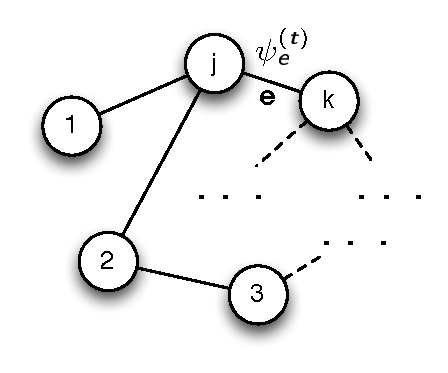
\includegraphics[scale=0.35]{./ensemble_2.pdf}
		\end{figure}		$\{\psi^{(t)}_e(x,++),\psi^{(t)}_e(x,+-),\psi^{(t)}_e(x,-+),\psi^{(t)}_e(x,--)\}$
	Prediction is by $\hat\yb(x) = \argmax_{\yb \in \Ycal}\sum_e \psi_e(x,\yb_e) $.

	% ensemble 1
	\vspace{0.1cm}
	\normalsize{\color{sciorange} MAJORITY VOTING ENSEMBLE (MVE)}\\
	\footnotesize
	In MVE, the ensemble prediction or each microlabel is the most frequently appearing prediction among the base classifiers 
	\begin{align*}
	F_{j}^{\text{\tiny MVE}}(x) = \argmax_{y_j \in \Ycal_j} \left(\frac{1}{T} \sum_{i=1}^T \ind{F_{j}^{(t)}(x)=y_j}\right),
	% \label{ensemble1}
	\end{align*}
	where $F^{(t)}(x) = (F_j^{(t)}(x))_{j=1}^k$ is the predicted multilabel in $t$'th base classifier.

	% ensemble 2
	\vspace{0.1cm}
	\normalsize{\color{sciorange} AVERAGE OF MAX-MARGINALS (AMM)}\\
	\footnotesize
	\begin{figure}[t]
	\vspace{-4mm}
	\begin{center}
		\includegraphics[page={1},width=1 \columnwidth]{./ensemble_2a.pdf}
	\label{ensemble_3}
	\end{center}
	\end{figure}
	\vspace{-5mm}
	Our goal is to infer for each microlabel $u$ of each node $j$
	its {\em max-marginal}, that is, the maximum score of a multilabel that is consistent with $y_j = u_j, \, u_j\in\{+,-\}$
	\begin{align*}
	{\tilde\psi}_{j}(x,u_j) &= \underset{\{\yb \in \Ycal:y_j= u_j\}}{\mathbf{\maximize}} \sum_e \psi_e(x,\yb_e). \label{eg_global} 
	\end{align*}
	
	The ensemble prediction for each target is obtained by averaging the max-marginals  of the base models and choosing the maximizing microlabel for the node:
	\begin{align*}
	F^{\text{\tiny AMM}}_j(x) = \underset{u_j \in \Ycal_j}{\argmax} \frac{1}{|T|} \sum_{t=1}^{T}{\tilde\psi}_{j,u_j}^{(t)}(x),% \label{ensemble2},
	\end{align*}
	and the predicted multilabel is composed from the predicted  microlabels
	\begin{align*}
	F^{\text{\tiny AMM}}(x) = \left(F^{\text{\tiny AMM}}_j(x)\right)_{j \in V}.
	\end{align*}
	

	% ensemble 3
	\vspace{0.1cm}
	\normalsize{\color{sciorange} MAXIMUM AVERAGE MARGINALS (MAM)}\\
	\footnotesize
	Generate the {\bf union graph} of the trees underlying the base models, with average edge labeling scores $\frac{1}{|T_e|} \sum_{t  \in T(e) } \psi^{(t)}_{e,u}(x)$ (normalized by how many times an edge appears)
	\begin{figure}[t]
	\vspace{-2mm}
	\begin{center}
		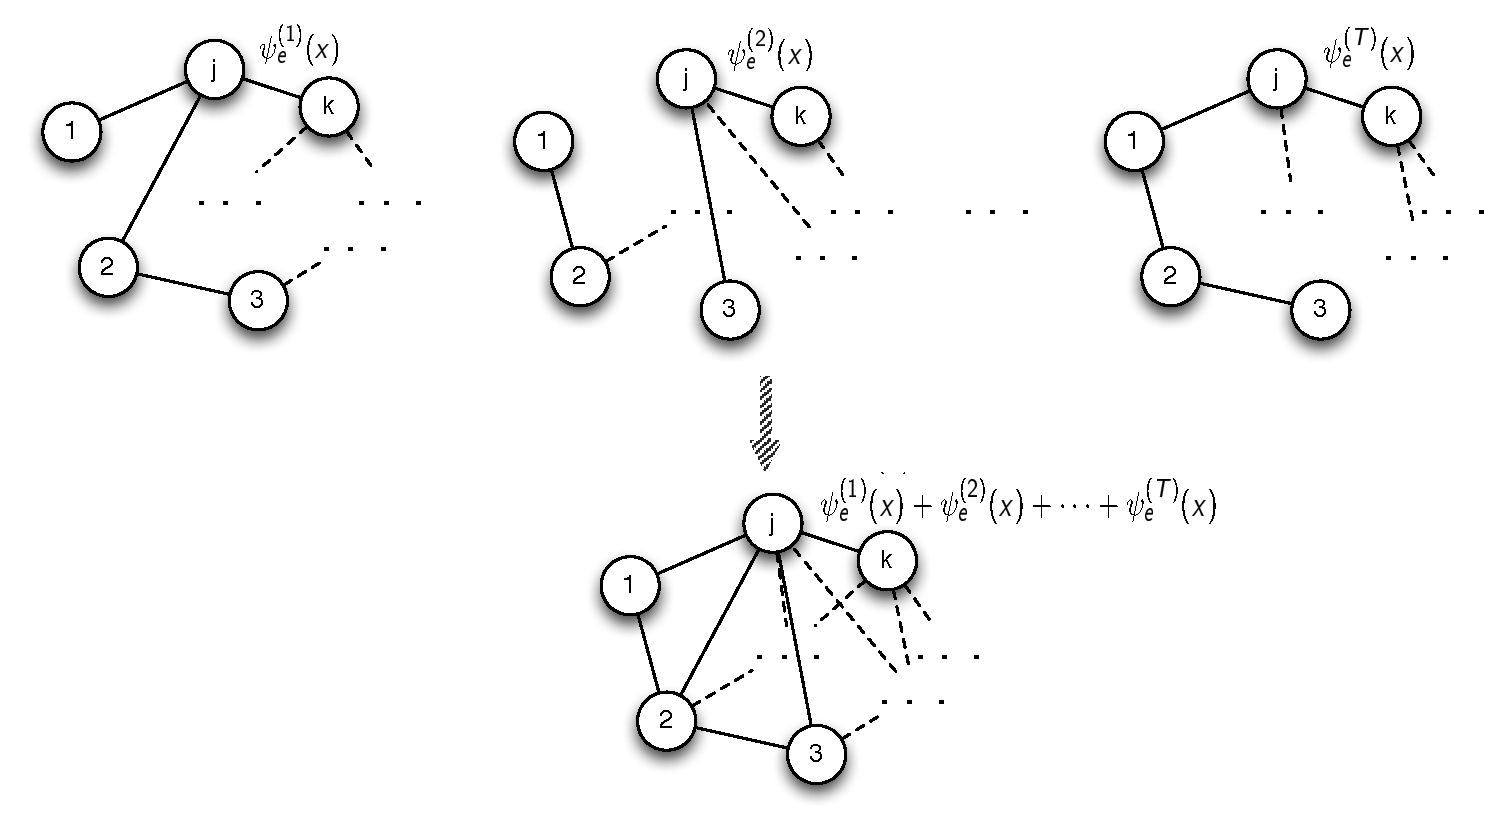
\includegraphics[page={1},width=1 \columnwidth]{./ensemble_3.pdf}
	\label{ensemble_3}
	\end{center}
	\end{figure}
	\vspace{-5mm}
	Inference on the union graph:
		\begin{align*}
			F^{\text{\tiny MAM}}(x) &= \underset{\yb \in \Ycal }{\argmax}\,\sum_{e\in \cup_t E_t}\frac{1}{T}\sum_{t=1}^{T}\ \psi^{(t)}_e(x,\yb_e)
		\end{align*}			
	Interpretation: ensemble prediction is the multilabel maximizing the average score over the base models.
	


	\end{multicols}
\end{textblock}

%-------------------+
%	middle right	|
%-------------------+
\begin{textblock}{137}(63,128)
	\sffamily
	\Large{\color{sciorange}EXPERIMENTAL RESULTS}\small\\
	\rule[3mm]{137mm}{0.1pt}
	
	\vspace{-4mm}	
	
	\begin{figure}[t]
	\vspace{-5mm}
	\begin{center}
		\caption{Ensemble learning curve (microlabel accuracy) plotted as the size of ensemble. Average performance of base learner with random tree as output graph structure is denoted as horizontal dash line.}
		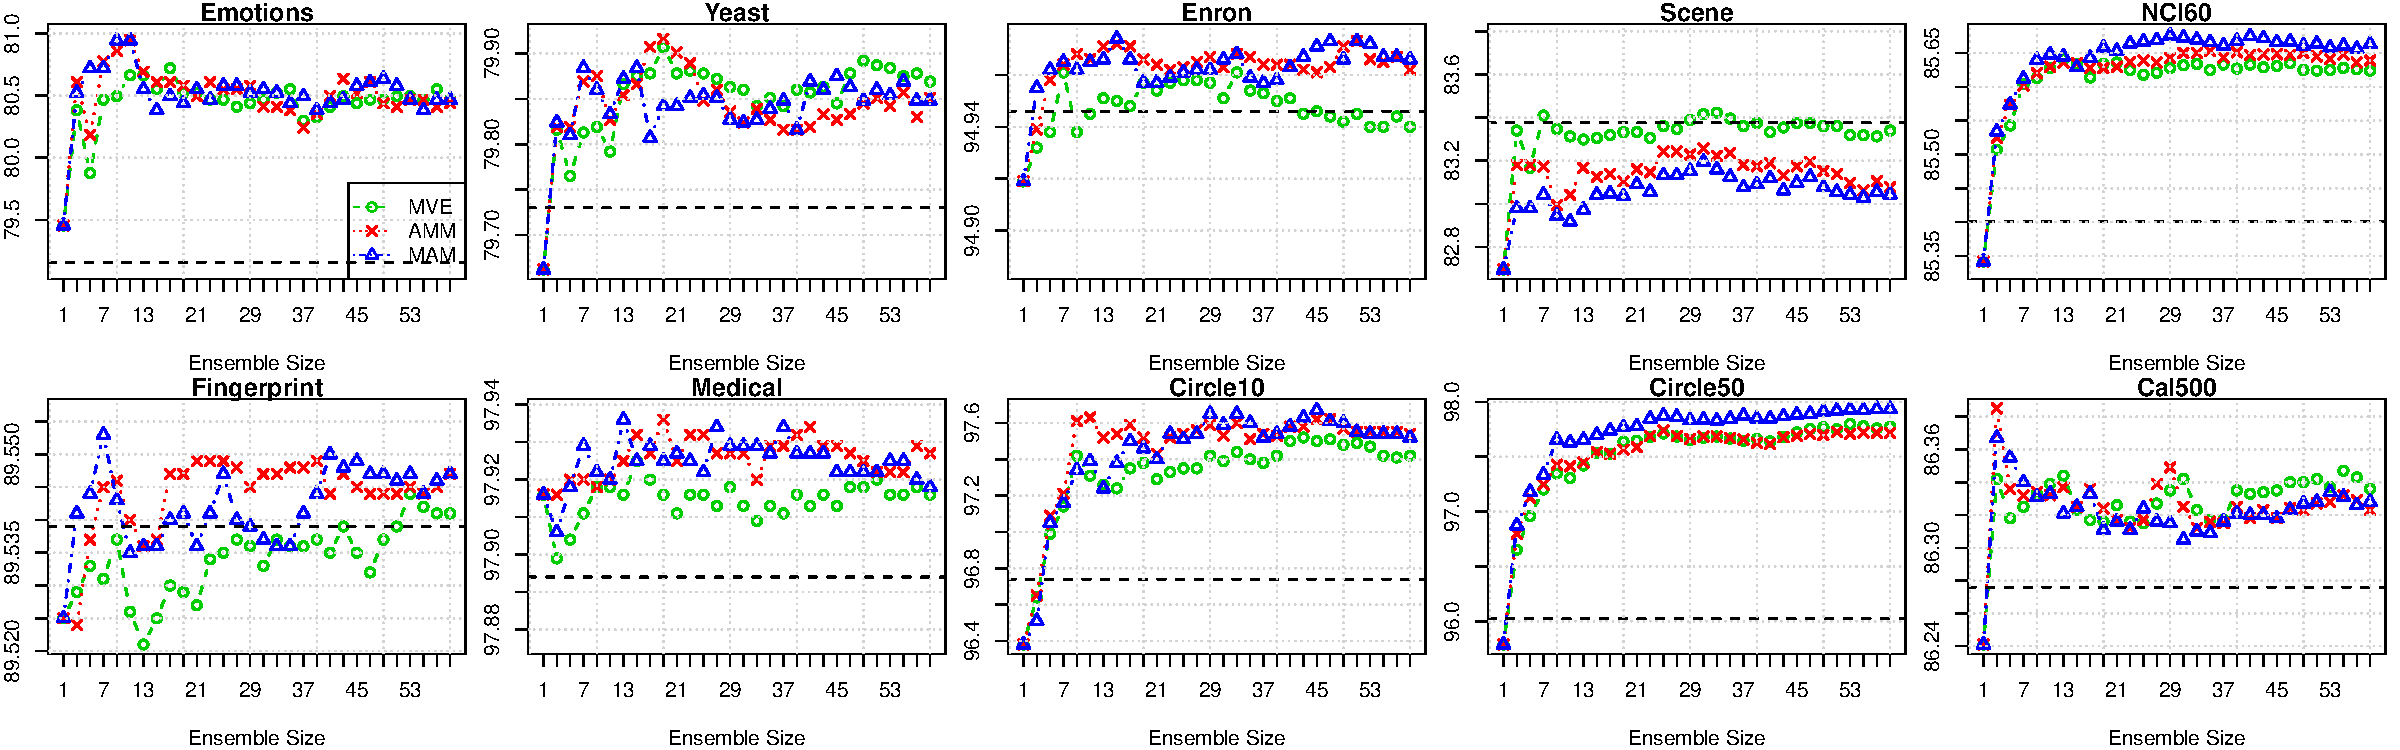
\includegraphics[page={1},width=1 \columnwidth]{./ensemble_curve.pdf}
	\label{ensemblemethodeffect}
	\end{center}
	\end{figure}
	
	\vspace{-14mm}
	
	\begin{multicols}{2}
	\begin{table}
		\small
		\caption{Prediction performance by microlabel accuracy.}
			\vspace{-5mm}
		\label{prediction_performance_1}
		\begin{center}
		\begin{tiny}
		\begin{sc}
		\begin{tabular}{|p{0.65cm}|p{0.52cm}|p{0.55cm}|p{0.68cm}|p{0.52cm}|p{0.55cm}|p{0.52cm}|} \hline
			\multirow{2}{*}{\textbf{Dataset}} 
			& \multicolumn{6}{c|}{\textbf{Microlabel Accuracy}} \\ \cline{2-7} 
		    & Svm & Bagging & AdaBoost & Mtl & Mmcrf & Mam\\ \cline{1-7}
			Emotions & {77.3}$\pm${1.9} & {74.1}$\pm${1.8} & {76.8}$\pm${1.6} & \em{79.8}$\pm${1.8} & {79.2}$\pm${0.9} & \bf{80.5}$\pm${1.4} \\ \hline
			Yeast & \bf{80.0}$\pm${0.6} & {78.4}$\pm${0.7} & {74.8}$\pm${0.3} & {79.3}$\pm${0.2} & {79.7}$\pm${0.3} & \em{79.9}$\pm${0.4} \\ \hline
			Scene & \bf{90.2}$\pm${0.3} & {87.8}$\pm${0.8} & {84.3}$\pm${0.4} & \em{88.4}$\pm${0.6} & {83.4}$\pm${0.2} & {83.0}$\pm${0.2} \\ \hline
			Enron & {93.6}$\pm${0.2} & {93.7}$\pm${0.1} & {86.2}$\pm${0.2} & {93.5}$\pm${0.1} & \em{94.9}$\pm${0.1} & \bf{95.0}$\pm${0.2} \\ \hline
			Cal500 & \bf{86.3}$\pm${0.3} & {86.0}$\pm${0.2} & {74.9}$\pm${0.4} & {86.2}$\pm${0.2} & \bf{86.3}$\pm${0.2} & \bf{86.3}$\pm${0.3} \\ \hline
			FP & \bf{89.7}$\pm${0.2} & {85.0}$\pm${0.7} & {84.1}$\pm${0.5} & {82.7}$\pm${0.3} & \em{89.5}$\pm${0.3} & \em{89.5}$\pm${0.8} \\ \hline
			NCI60 & {84.7}$\pm${0.7} & {79.5}$\pm${0.8} & {79.3}$\pm${1.0} & {84.0}$\pm${1.1} & \em{85.4}$\pm${0.9} & \bf{85.7}$\pm${0.7} \\ \hline
			Medical & {97.4}$\pm${0.1} & {97.4}$\pm${0.1} & {91.4}$\pm${0.3} & {97.4}$\pm${0.1} & \bf{97.9}$\pm${0.1} & \bf{97.9}$\pm${0.1} \\ \hline
			Circle10 & {94.8}$\pm${0.9} & {92.9}$\pm${0.9} & \bf{98.0}$\pm${0.4} & {93.7}$\pm${1.4} & {96.7}$\pm${0.7} & \em{97.5}$\pm${0.3} \\ \hline
			Circle50 & {94.1}$\pm${0.3} & {91.7}$\pm${0.3} & \em{96.6}$\pm${0.2} & {93.8}$\pm${0.7} & {96.0}$\pm${0.1} & \bf{97.9}$\pm${0.2} \\ \hline
			$@Top2$ & {4} & {0} & {2} & {2} & \em{5} & \bf{9} \\ \hline
		\end{tabular}
		\end{sc}
		\end{tiny}
		\end{center}
	\end{table}	


	\begin{table}
		\small
		\caption{Prediction performance by multilabel accuracy.}
			\vspace{-5mm}
		\label{prediction_performance_2}
		\begin{center}
		\begin{tiny}
		\begin{sc}
	\begin{tabular}{|p{0.65cm}|p{0.52cm}|p{0.55cm}|p{0.68cm}|p{0.52cm}|p{0.55cm}|p{0.52cm}|} \hline
			\multirow{2}{*}{\textbf{Dataset}} 
			& \multicolumn{6}{c|}{\textbf{Multilabel Accuracy}} \\ \cline{2-7} 
		    & Svm & Bagging & AdaBoost & Mtl & Mmcrf & Mam\\ \cline{1-7}
			Emotions & {21.2}$\pm${3.4} & {20.9}$\pm${2.6} & {23.8}$\pm${2.3} & {25.5}$\pm${3.5} & \em{26.5}$\pm${3.1} & \bf{30.4}$\pm${4.2} \\ \hline
			Yeast & \em{14.0}$\pm${1.8} & {13.1}$\pm${1.2} & {7.5}$\pm${1.3} & {11.3}$\pm${2.8} & {13.8}$\pm${1.5} & \bf{14.0}$\pm${0.6} \\ \hline
			Scene & \bf{52.8}$\pm${1.0} & \em{46.5}$\pm${2.5} & {34.7}$\pm${1.8} & {44.8}$\pm${3.0} & {12.6}$\pm${0.7} & {5.4}$\pm${0.5} \\ \hline
			Enron & {0.4}$\pm${0.1} & {0.1}$\pm${0.2} & {0.0}$\pm${0.0} & {0.4}$\pm${0.3} & \em{11.7}$\pm${1.2} & \bf{12.1}$\pm${1.0} \\ \hline
			Cal500 & {0.0}$\pm${0.0} & {0.0}$\pm${0.0} & {0.0}$\pm${0.0} & {0.0}$\pm${0.0} & {0.0}$\pm${0.0} & {0.0}$\pm${0.0} \\ \hline
			FP & \bf{1.0}$\pm${1.0} & {0.0}$\pm${0.0} & {0.0}$\pm${0.0} & {0.0}$\pm${0.0} & \em{0.4}$\pm${0.9} & \em{0.4}$\pm${0.5} \\ \hline
			NCI60 & \em{43.1}$\pm${1.3} & {21.1}$\pm${1.3} & {2.5}$\pm${0.6} & \bf{47.0}$\pm${1.4} & {36.9}$\pm${0.8} & {40.0}$\pm${1.0} \\ \hline
			Medical & {8.2}$\pm${2.3} & {8.2}$\pm${1.6} & {5.1}$\pm${1.0} & {8.2}$\pm${1.2} & \em{35.9}$\pm${2.1} & \bf{36.9}$\pm${4.6} \\ \hline
			Circle10 & {69.1}$\pm${4.0} & {64.8}$\pm${3.2} & \bf{86.0}$\pm${2.0} & {66.8}$\pm${3.4} & {75.2}$\pm${5.6} & \em{82.3}$\pm${2.2} \\ \hline
			Circle50 & {29.7}$\pm${2.5} & {21.7}$\pm${2.6} & {28.9}$\pm${3.6} & {27.7}$\pm${3.4} & \em{30.8}$\pm${1.9} & \bf{53.8}$\pm${2.2} \\ \hline
			$@Top2$ & {5} & {2} & {2} & {2} & \em{6} & \bf{8} \\ \hline
		\end{tabular}
		\end{sc}
		\end{tiny}
		\end{center}
	\end{table}	

	\end{multicols}
\end{textblock}



\end{document}
